% !TeX spellcheck = de_DE
\documentclass[12pt,a4]{article}

\usepackage{graphicx}
\usepackage{amssymb}%math symbols
\PassOptionsToPackage{hyphens}{url}\usepackage{hyperref}%allows urls to follow line breaks of text
\usepackage{xcolor}
\usepackage{comment}
\usepackage[german]{babel}%allos usage of vowel mutations
\usepackage{wrapfig} %allows text to wrap images
\usepackage{multicol}%allos multi column text formatting



\usepackage[utf8]{inputenc}%implements vowel mutations
\raggedright %shifts text to the left page border


%\begin{comment}

%sets colors for links
\hypersetup{
	colorlinks=false,
	urlbordercolor=red,
	%urlcolor=red,
	%linkcolor=red,
	%filecolor=red,      
	%urlcolor=red,
	pdftitle={Programmierung von Systemen},
	%bookmarks=true,
	%pdfpagemode=FullScreen,
}
%\end{comment}
%the figure element allows you to insert a logo on the title page
\title{
	\begin{figure}
		\centering
		
\includegraphics[height=1.5cm]{logo.png}
	\end{figure}
Programmierung von Systemen 
}

\author{Erik Neller | Dozent: Matthias Tichy}
%\date{18.08.2020}

\begin{document}
	
	\maketitle
	\thispagestyle{empty} %removes page number from title
	\newpage
	
	\tableofcontents
	\newpage
	

	\section{UML-Klassendiagramme}
	\subsection{Klassen und Schnittstellen}
	Methoden und Attribute werden wie in Java in der Form \texttt{\$TYP \$NAME} angegeben, ist die Methode vom Typ \texttt{void} entfällt der Rückgabetyp.
	\begin{itemize}
		\item \texttt{private} wird durch ''-'' symbolisiert
		\item \texttt{package} wird durch ''{\raise.17ex\hbox{$\scriptstyle\sim$}}'' symbolisiert
		\item \texttt{protected} wird durch ''\#'' symbolisiert
		\item \texttt{public} wird durch ''+'' symbolisiert
		\item \texttt{static}  wird \underline{unterstrichen}
	\end{itemize}
	\texttt{\{readonly\}} ist ein UML Attribut das für Konstanten verwendet wird. 
	\newline\newline
	
	Der Block einer Klasse / eines Interfaces besteht aus drei Feldern: 
	\begin{enumerate}
		\item Name mit Modifikatoren
		\item Attribute (Variablen)
		\item Methoden
	\end{enumerate}
	 Modifikatoren für die Klasse können sein: \texttt{\flqq interface\frqq} oder \texttt{\{abstract\}} bzw. der Name in \textit{kursiv}.
	 
	 Die Multiplizität wird genutzt um Listen und Mengen von Objekten anzugeben, aber auch in Relationen zwischen Klassen:
	 \begin{center}
	 	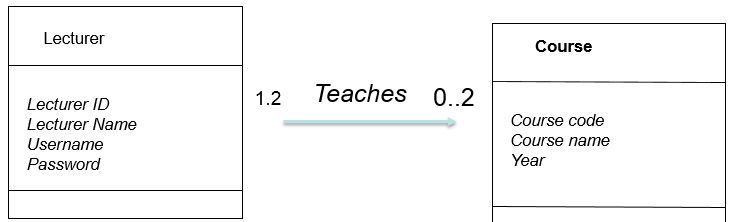
\includegraphics[width=0.5\linewidth]{images/multiplicity}
	 \end{center}
	 \begin{enumerate}
	 	\item Typ
	 	\item Größe begrenzt \{1..x\} oder unendlich [*]
	 	\item Attribute wie \{order\} und \{unique\}
	 \end{enumerate}

	 \subsection{Relationen}

 	\texttt{extends} oder \texttt{implements} wird dargestellt durch einen nicht ausgefüllten Pfeil, wobei die Linie bei gleichen Typen (Interface erbt von Interface, Klasse von Klasse) durchgezogen ist, wenn eine Klasse ein Interface implementiert, gestrichelt.
 	
 	\begin{center}
 		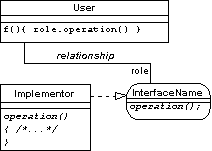
\includegraphics[width=0.5\linewidth]{images/interface1}
 	\end{center}

		
	 
	 \begin{itemize}
	 	\item Abhängigkeit (Dependency): User nutzt Ressource, aber die Ressource ist nicht Teil der User Klasse. Wird die Ressource modifiziert, muss auch der User modifiziert werden. 
	 		\begin{center}
	 		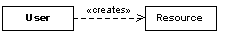
\includegraphics[width=0.5\linewidth]{images/dependency}
	 		\end{center}
 		
 		\item Aggregation: ''ist Teil von'', wird symbolisiert durch einen Pfeil mit leerer Raute
	 	\begin{center}
	 		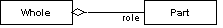
\includegraphics[width=0.5\linewidth]{images/aggregation}
	 	\end{center}
	 	
	 	\item Komposition ''besteht aus'', wird symbolisiert durch einen Pfeil mit ausgefüllter Raute
	 	\begin{center}
	 		
\includegraphics[width=0.5\linewidth]{images/composition}
	 	\end{center}
 	
 		\item Assoziation: Die Klassen sind auf eine beliebige Weise verbunden, nutzen Methoden der anderen aber nicht auf die oben genannten Weisen
 		\begin{center}
 			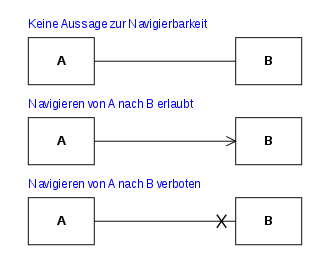
\includegraphics[width=0.4\linewidth]{images/association}
 		\end{center}
	 \end{itemize}
	
	Kommentare werden mit einer gestrichelten Linie mit dem eigentlichen Objekt verbunden.
	
	
	\section{Version Control Systems}

	\subsection{Grundlegende Funktionen}
		Version Control Systems (VCS) erlauben die Verwaltung von mehreren Teilen und Versionen eines Projekts und damit die Zusammenarbeit von mehreren Teilnehmern.
	\begin{itemize}
		\item Rechteverwaltung (z.B. Entwickler von Front-und Backend, Projektmanagement)
		\item Archivierung in verschiedenen Versionen (einfach anhand der gemachten Änderung, anstatt vollständige Backups zu machen)
		\item Speicherung von Metadaten: Historie von Änderungen mit Datum, Autor, etc.
		\item Backup zur Wiederherstellung lokal gelöschter Daten oder versehentlicher Änderungen
		\item Zentralisierung auf Server
		
	\end{itemize}
	\subsection{Git}
	Das Git System besteht aus vier Teilen, von denen drei durch Git selbst implementiert werden. Jede Änderung durchläuft sie in dieser Reihenfolge: 
	\begin{enumerate}
		\item Der eigentlichen Arbeitsplatz / \textit{Workspace} in dem Änderungen an Dateien vorgenommen werden
		\item Die \textit{staging area}, in der \textit{commits} aus einzelnen Änderungen an Dateien feingranular (bis zu einzelnen Zeilen) zusammengesetzt werden
		\item Das \textit{lokalen Repository}
		\item Das \textit{remote Repository} auf einem Server, beispielsweise GitHub oder GitLab
	\end{enumerate}
	Auf den einzelnen Bereichen existieren verschiedene Befehle. Für die staging area:
	\begin{itemize}
		\item \texttt{git init} erstellt ein neues Git-Repository im aktuellen Verzeichnis
		\item \texttt{git add} um Dateien der staging area hinzuzufügen
		\item In einer \texttt{.gitignore} Datei können Regeln für Dateien angegeben werden, die generell nicht mit in die staging area aufgenommen werden sollen
		\item \texttt{git status} um aktuell geänderte und getrackte Dateien zu sehen
		\item \texttt{git rm --cached} um Dateien aus der staging area zu entfernen
		
	\end{itemize}
	%\newline
	Für das lokale Repository:
	\begin{itemize}
		\item \texttt{git commit -m \$MESSAGE} um den Inhalt der staging area in das lokale Repository hinzuzufügen
		\item \texttt{git checkout \$COMMIT-HASH} erlaubt das Wiederherstellen vorheriger Zustände von commits
		\item \texttt{git reset --soft HEAD{\raise.17ex\hbox{$\scriptstyle\sim$}}x} erlaubt das Rückgängigmachen von x commits
		\item \texttt{git log} zeigt den Verlauf von commits an
		\item \texttt{git remote add \$NAME \$ADDRESS} verknüpft das lokale Repository mit einem remote Repository
	\end{itemize}

	Und für das remote Repository:
	\begin{itemize}
		\item \texttt{git push \$REPOSITORY \$BRANCH} um den lokalen commit auf den Server zu legen
		\item \texttt{git pull} um das lokale Repository mit den Änderungen aus dem remote Repository zu aktualisieren
		\item \texttt{git clone \$REPOSITORY} um das ganze Repository lokal zu speichern
	\end{itemize}


	
	Für verschiedene Themengebiete / Zuständigkeitsbereiche existiert das Konzept von Branches(Verzweigungen), die mit \texttt{git branch \$NAME} erstellt werden können, um anschließend mit \texttt{git checkout \$NAME} in den Branch zu wechseln, oder in Kurzform: \texttt{git checkout -b \$NAME}. Mit \texttt{git merge \$NAME} kann dann ein Branch in den jeweils Aktuellen integriert, oder mit \texttt{git branch -d \$NAME} gelöscht werden. Ist keine automatische Vereinigung der Branches möglich, müssen die angezeigten Dateien manuell geändert und anschließend mit \texttt{git add \$FILE} Alternativ kann der Branch in das Repository aufgenommen werden: \texttt{git push \$REMOTE \$BRANCH}.
	
	
	


	\section{Objektorientierung}
	\subsection{Interfaces}
	Analog zur abstrakten Klasse erlaubt ein Interface keine Instanziierung. Es enthält keine tatsächliche Implementierung, sondern nur Methodenrümpfe und evtl. Konstanten und muss dementsprechend in jeder Klasse mit dem Schlüsselwort \texttt{implements} implementiert werden. Im Gegensatz zu abstrakten Klassen können mehrere Interfaces von einer Klasse implementiert werden.
	
	\subsection{Sichtbarkeit}
	
	\begin{center}
		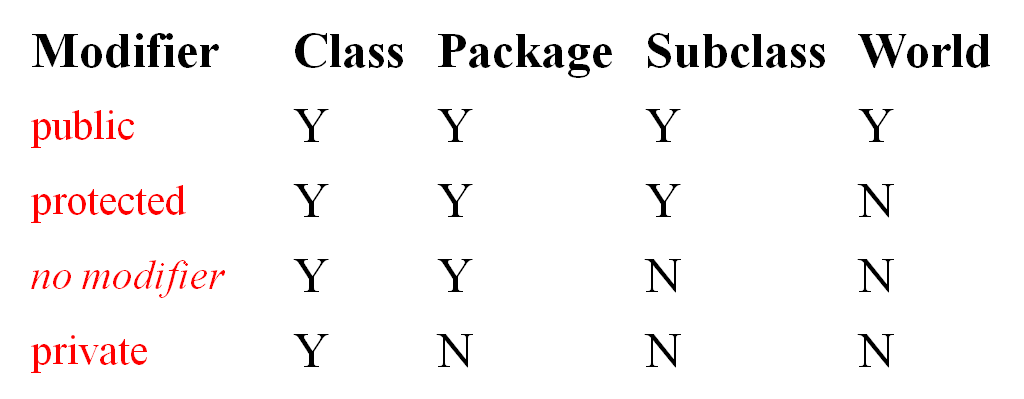
\includegraphics[width=0.7\linewidth]{images/modifiers}
	\end{center}
	
	
	\subsection{Annotations}
	Verschiedene Standardannotationen, eigene definierbar. Durch Reflection zur Laufzeit auslesbar.
	\begin{itemize}
		\item \texttt{@Override} gibt an dass hier ein Element überschrieben werden soll
		\item \texttt{@Deprecated} gibt eine Warnung aus dass Element veraltet ist
		\item \texttt{@SuppressWarnings()} unterdrückt die angegebene Warnung
		\item \texttt{@Documented} nimmt nachfolgende Annotationen in die JavaDoc mit auf
	\end{itemize}
	JavaDoc:
	\begin{itemize}
		\item \texttt{@author}
		\item \texttt{@version}
		\item \texttt{@param} zur Beschreibung von Methodenparametern
		\item \texttt{@return} beschreibt den Rückgabewert
		\item \texttt{@exception}, \texttt{@throws} Beschreibt Fehlermeldungen, die diese Methode produzieren kann
		\item \texttt{@link} Verknüpfung zu anderem Symbol
	\end{itemize}
	
	\subsection{Enumerations}
	Mit einem \texttt{enum} kann eine Menge von Konstanten definiert werden, entweder auf Klassenlevel oder innerhalb einer Klasse. Sie sind auch selbst eine Klasse, deren Attribute \texttt{public static final} definiert sind. Methoden: 
	\begin{itemize}
		\item \texttt{int ordinal()} gibt die Position in der Liste des Enums zurück
		\item \texttt{String name()} gibt den Namen der Konstanten zurück
		\item \texttt{int valueOf} gibt den zugeordneten Wert der Variablen zurück 
	\end{itemize}
	
	\section{Collections}
	\subsection{Datenstrukturen}
	\subsubsection{Array}
	Statische Größe, wird mit Länge und Datentyp gespeichert, zB int[5]. Objekt x erhalten: array[x]. Länge: array.length
	\subsubsection{ArrayList}
	Klasse die zur Speicherung Arrays verwendet, diese aber ersetzt wenn die Methoden \texttt{add()} oder \texttt{remove()} aufgerufen werden. Mit \texttt{toArray()} kann der Array erhalten werden, mit \texttt{size()} die Größe, da diese dynamisch ist. Objekt erhalten: arraylist.get(x).
	\subsubsection{Linked List}
	Jedes Listenelement enthält einen Zeiger auf das nächste Element, bei dem letzten Element ist der Zeiger \texttt{NULL}.
	\subsubsection{Double Linked List}
	Wie linked list, nur dass jedes Element zusätzlich einen Zeiger auf das vorherige Element enthält (beim ersten Element \texttt{NULL}).
	\subsubsection{Sorted Tree}
	Setzt die Sortierbarkeit der Objekte voraus: Objekte mit kleinerem Wert sind links des Vaterknotens, mit größerem rechts. Beim Einfügen / Entfernen reorganisieren: rot-schwarz Bäume, B Baum, B+Baum
	\begin{center}
		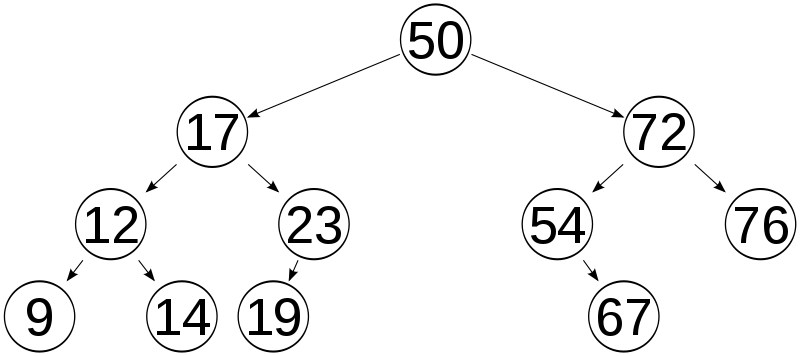
\includegraphics[width=0.5\linewidth]{images/sortedtree}
	\end{center}
	\subsubsection{HashTable}
	Objekte werden gehasht, also ein Wert aus ihnen berechnet, anhand dessen sie in in eine Tabelle eingeordnet werden.
	\subsubsection{Map}
	Speichert nicht einzelne Werte, sondern Tupel aus (Key, Value), nutzt dann zB eine Liste aus Tupeln oder eine Hashtabelle anhand der Keys.
	
	\subsection{Collections API}
	Stellt effiziente Datenstrukturen für viele Anwendunge bereit, sodass Datenstrukturen und Algorithmen nicht selbst implementiert werden müssen.
	Das Collection Interface selbst enthält Methoden wie add(), size(), contains(), remove()
	\begin{itemize}
	
	\item List ist eine geordnete Collection: add(e), add(index, e), indexOf(e), contains(e) 
	\item Set ist eine Collection ohne Duplikate(inklusive \texttt{NULL}): add(), contains()
	\end{itemize}
	\subsection{Queue}
	Warteschlange als Datenstruktur bei der Elemente am einen Ende angehängt und am anderen Ende gelesen werden. Dementsprechend existieren die folgenden Methoden, die eine Exception verursachen bei Fehlern:
	
	\begin{itemize}
		\item add(e) fügt ein Element hinten an der Queue an, falls max. Größe erreicht Exception
		\item remove() nimmt das vorderste Element der Queue und gibt es zurück, gleichzeitig wird es aus der Queue entfernt (Exception falls Queue leer)
		\item element() gibt das erste Element aus der Queue zurück aber löscht es nicht (ebenfalls Exception falls leer)
	\end{itemize}

	Alternativ existieren die Methoden mit speziellen Rückgabewerten anstelle von Exceptions:
	\begin{itemize}
		\item offer(e) gibt true/false zurück ob Element hinzugefügt wurde
		\item poll() gibt Element oder \texttt{NULL} zurück
		\item peek() gibt Element oder \texttt{NULL} zurück
	\end{itemize}

	\subsection{Deque}
	Ist die Erweiterung einer Queue mit den gleichen Operationen an beiden Enden der Datenstruktur, analog zu einem Kartendeck (daher auch oft fälschlich Dequeue geschrieben: Double Ended queue)
	
	\subsubsection{Exception und special Element}
	
\begin{tabular}{|c|c|c|c|c|}
	\hline 
	&\multicolumn{2}{|c|}{\textbf{throw Exception}}&\multicolumn{2}{|c|}{\textbf{special Element}} \\
	\hline 
	&\textit{first}&\textit{last}&\textit{first}&\textit{last}  \\ 
	\hline 
	\textbf{einfügen}&addFirst()&addLast()&offerFirst()&offerLast()\\ 
	\hline 
	\textbf{löschen}&  removeFirst()&removeLast()&pollFirst()&pollLast()\\ 
	\hline 
	\textbf{lesen}(behalten)&getFirst()&getLast()&peekFirst()&peekLast()\\ 
	\hline 
\end{tabular} 

	\subsubsection{Blocking Deque}
	Die dritte Möglichkeit ist, den Thread zu blockieren wenn die Operation nicht möglich ist. Davon existieren zwei Varianten: mit maximaler Blockierungszeit (Timeout) und ohne. Dieses blocking deque implementiert sowohl die blocking Queue (welche queue und blocking implementiert) als auch das Deque.
	\begin{center}
	\begin{tabular}{|c|c|c|}
		\hline 
		&\textbf{block}&\textbf{timeout}\\ 
		\hline 
		\textbf{einfügen}&putFirst()&offerFirst(e,time,unit)\\ 
		\hline 
		\textbf{löschen}&takeFirst()&pollFirst(e,time,unit)\\ 
		\hline 
		\textbf{lesen}(behalten)&-&-  \\ 
		\hline 
	\end{tabular} 
	\end{center}
	\subsection{Generics}
	Collections können \textit{generisch} verwendet werden, indem bei der Initialisierung eine Klasse angegeben wird, deren Instanzen in der Collection enthalten sein werden. Bei allen anderen Klassen / Datentypen wird der Compiler hier direkt eine Fehlermeldung liefern, was der Alternative, potenzielle Fehler während der Laufzeit, vorzuziehen ist.
	\subsection{Streams}
	Streams aus \texttt{java.util.stram.Stream<T>} stellen Ströme von Referenzen dar, die es erlauben, verkettete Operationen auf diesem Datenstrom nacheinander oder parallel auszuführen. Bestimmte Methoden erlauben die Verwendung von Prädikaten und klassischen mathematischen Funktionen. Wo vorher eine for-Schleife mit Zählvariable notwendig war um die Anzahl von bestimmten Elementen in einem Array zu erhalten, kann man damit schreiben: \texttt{anzahl = Arrays.stream(myArray).filter(x -> x.equals("String")).count();}
	
	\section{Java IO}
	\subsection{Streams}
	Grundlegende Operationen beim Lesen von Daten: 
	\begin{itemize}
		\item read
		\item skip
		\item available (prüfen ob Daten verfügbar)
		\item close
	\end{itemize}
	und beim schreiben von Daten: 
	\begin{itemize}
		\item write
		\item flush (prüfen ob richtig geschrieben)
		\item close
	\end{itemize}

	Verschiedene Arten von Daten die in Java gelesen werden: ByteArray, Object, andere Dateien
	
	Ein Stream ist  eine ''Hülle'' für eine Datei und kann wie der utilStream mehrere Dateien als kontinuierlichen Strom bearbeiten.
	
	Für die verschiedene Zwecke existieren auch verschiedene Streams, die einander übergeben werden können:
	\begin{itemize}
		\item InputStream als generelles Interface / Klasse
		\item FileInputStream zum Lesen von Dateien
		\item ByteArrayInputStream zum Lesen von ByteArrays
		\item DataInputStream zum Lesen von Java Datentypen
		\item ObjectInputStream zum Lesen von Java Objekten (Problem: Versionierung)
		\item SequenceInputStream zum Verknüpfen mehrerer Inputstreams
		\item BufferedInputStream zum schnelleren Lesen über einen Pufferspeicher
	\end{itemize}
\subsection{Reader/Writer}
	Liest statt Bytes lesbare Zeichen/Characters, also ist ein Reader/writer eine erweiterte Version der Streams der zusätzlich eine Übersetzung von Characters in Bytes macht.
	\begin{itemize}
		\item Reader
		\item FileReader
		\item StringReader analog zu ByteArrayInputStream
		\item BufferedReader
		\item InputStreamReader um von Stream zu Reader zu übersetzen
	\end{itemize}
Über ein boolean flag kann außerdem bestimmt werden, ob an die existierende Datei beim Schreiben angehängt werden soll. Tatsächlich wahlfreien Zugriff erhält man mit RandomAccessFile(file,mode), das dann auch die Methoden seek() und getFilePointer() bereitstellt. Zur Erleichterung der Nutzung existiert außerdem das try-with-resources-Statement.
\subsection{Decorator Pattern}
Reader / Writer und Streams nutzen das Decorator Pattern um die Kombination verschiedener Funktionalitäten zu erleichtern. Anstatt BufferedDataFileInputStream zu implementieren, können einfach die verschiedenen Streams einander übergeben werden und so ''verschachtelt'' verwendet werden. Im Decorator Pattern werden die grundlegenden Methoden, die von der konkreten Komponente und den Decoratorn implementiert werden, durch ein Interface definiert. Jede Decorator Klasse kann dann unter Verwendung der konkreten Komponente zusätzliche Funktionen hinzufügen.
\begin{center}
	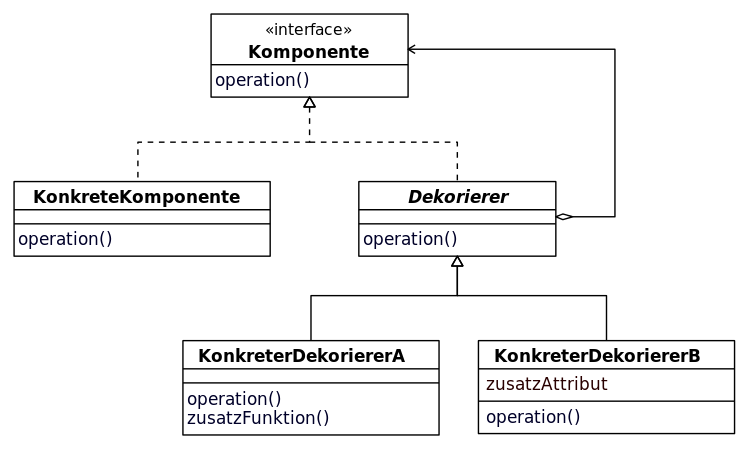
\includegraphics[width=0.5\linewidth]{images/decorator}
\end{center}


\section{Dateien}
\subsection{java.io.file}
In java.io.file sind sämtliche Java-Methoden zum Umgang mit Dateien zusammengefasst.
\subsection{java.nio.file.*}
Stellt erneuerte, sortierte Methoden zum Umgang mit Dateien bereit.
\begin{itemize}
	\item FileSystem(s): Wurzelverzeichnisse / Arten von Dateisystemen
	\item Path(s): Pfade zu Dateien / Verzeichnissen
	\item Files: zur tatsächlichen Manipulation von Dateien
\end{itemize}
\subsection{Scanner}
Kann primitive Typen scannen: Boolean, int, Double, String.
Mit den Methoden hasNext kann überprüft werden ob der Scanner eine Eingabe des entsprechenden Typs bereit hält, um diesen dann mit next()  abzurufen.
\subsection{RegEx}
Reguläre Ausdrücke aus der Automaten - / Sprachentheorie können verwendet werden um Übereinstimmung mit einem Format zu prüfen.
 \subsubsection{Zeichenauswahl}
 Innerhalb von [] lässt sich eine Zeichenauswahl treffen.
 \begin{itemize}
 	\item \(\left[egh\right]\) wählt eines der Zeichen e,g oder h aus
 	\item \(\left[0-6\right]\) eine Zifer von 0 bis 6
 	\item \(\left[a-zA-Z0-9\right]\) lateinischer Buchstabe oder Ziffer
 	\item \(\left[\wedge a\right]\) negiert a, alles außer a
 \end{itemize}
 
 	Vordefinierte Zeichenklassen:
 	\begin{itemize}
 		\item \textbackslash d für digit, also Zahlsymbole
 		\item \textbackslash w word character inklusive Unterstrich \(\left[a-zA-Z_0-9\right]\), eventuell auch nicht-lateinische Buchstaben
 		\item \textbackslash s WhiteSpace
 		\item \textbackslash n newline
 		\item . (Punkt) als Wildcard für alle Zeichen außer Zeilenumbrüchen, im single-line mode auch diese
 	\end{itemize}
 Vordefinierte Zeichenklassen können mit der großgeschriebenen Variante negiert werden: während \textbackslash d für [0-9] steht, bedeutet \textbackslash D \(\left[\wedge 0-9\right]\).
 Die Zeichensätze, insbesondere die der Buchstaben, sind in der Regel von der Betriebssystem-locale abhängig.
	\subsubsection{Quantoren}
	
	\begin{center}
	\begin{tabular}{|c|c|c|c|c|c|c|c|}
		\hline 
		Ausdruck&  & ? & + & *&*?&\{m,n\}&\{m\}\\ 
		\hline 
		Bedeutung&  1&  0,1& \(\geq 1\) &  \(\geq 0\)&kleinste passende Zeichenkette&\{min,max\}&\{m,m\}\\ 
		\hline 
	\end{tabular} 
\end{center}

\subsubsection{Spezielle Zeichen}
\begin{itemize}
	\item \(\wedge\) Anfang der Zeile
	\item \$ Ende der Zeile
	\item X\textbar Z X oder Z
	\item XZ X gefolgt von Z
	\item () zum Gruppieren von Ausdrücken, kann später mit \$x wieder aufgerufen werden, Zählung beginnt mit 1; capture group
	\item (?:) um eine Zeichenkette zu gruppieren, aber nicht zu speichern (kann später nicht aufgerufen werden); non-capturing group
	\item a(?!b) a, wenn nicht gefolgt von b (negative lookahead)
	\item \textbackslash 1 um auf Capture Groups zuzugreifen, die dann den tatsächlichen Inhalt referenzieren.
	
%	https://www.keycdn.com/support/regex-cheatsheet
\end{itemize}
\subsubsection{Modi}
\begin{itemize}
	\item (?i) um Groß- und Kleinschreibung zu beachten
	\item (?s) für single-line Mode (ganze Datei als eine Zeile interpretieren)
	\item (?m) für multi-line mode
\end{itemize}
\subsubsection{Java}
Einige Java Funktionen unterstützen RegEx nativ, zB split(), matches(), replaceFirst(), replaceAll() aber \textbf{nicht} replace(). Außerdem existieren java-util.regex.Pattern und java.util.regex.Matcher .

\section{XML}
Extensible Markup Language zur Darstellung hierarchisch strukturierter Daten innerhalb einer Textdatei. 
Beginnt in der Regel mit \texttt{<?xml version=''1.0'' encoding=''UTF-8''?>}
Tags werden mit \texttt{\(<\)Tag\(>\) \textit{Inhalt} \(<\)/Tag\(>\)} angegeben und können Kind-Tags und Attribute haben. Kind-Tags werden innerhalb des Inhaltes angegeben, während Attribute im Tag selbst geschrieben werden, also \newline \texttt{\(<\)Tag attr="hello"\(>\) \textit{Inhalt} \(<\)/Tag\(>\)}. Um die Gültigkeit von XML Dateien sicherzustellen, muss ein Muster vorgegeben werden, mit dem diese geprüft werden kann. Die Syntax ist durch XML vorgegeben, die Gültigkeit der Kombinationen und des hierarchischen Aufbaus kann / muss jedoch je nach Anwendung angepasst werden und braucht dementsprechend eine variable Überprüfung.
Kommentare haben die Form \texttt{<!-- Kommentar -->}
\subsection{DTD}
\subsubsection{Verknüpfen}
Verwiesen wird auf die DTD in der XML Datei über \texttt{<!DOCTYPE \textit{rootNode} SYSTEM\textbar PUBLIC \textit{file.dtd}>}. Mit SYSTEM wird eine lokale URI angegeben, mit PUBLIC eine vordefinierte, online bereitgestellte DTD verwendet.
\subsubsection{Aufbau}
\begin{itemize}
	\item Element \texttt{<!ELEMENT Name Inhalt>}
	\item Attribut \texttt{<!ATTLIST referenzELement (Name Typ Wert)>} verschiedene Vorgaben für Attribute sind: \#REQUIRED, \#IMPLIED (=optional), \#FIXED, und ein Standardwert mit ''Wert''
	\item Entity \texttt{<!ENTITY name ''Zeichenkette''>} Abkürzung für einen String oder ein Dokument, das dann referenziert werden kann, also \#PCDATA
	
\end{itemize}

 Kindelemente werden nur mit Namen aufgezählt, nicht tatsächlich innerhalb der anderen Tags angegeben, da ein Tag auch mehrere Verwendungen haben könnte.

 Für die Angabe von Kindelementen existieren reguläre Ausdrücke:

Außerdem können Auflistungen in Reihenfolge durch Kommata getrennt werden und Elemente mit () gruppiert werden.
\subsubsection{Datentypen}
In einer DTD existieren nur zwei grundlegende Datentypen:
\begin{itemize}
	\item \#PCDATA, bei dem die Eingabe wie der Rest der Datei geparst wird, also in Text zum Beispiel \(<\)FETT\(>\) \(<\)/FETT\(>\) verwendet werden kann um verschiedene Formatierungen zu erhalten. Sollen in \#PCDATA reservierte Symbole verwendet werden, müssen deren Kodierungen statt der eigentlichen Symbole eingetragen werden.
	\item \#CDATA wird als reiner Text interpretiert
\end{itemize}
 
 
\subsection{XSD}%=DDDDDDDDDDDDDDDDDDDDDDDDDDDDDDDD
XML Schema Definition ist selbst in XML und verweist auf eine ''root'' XSD Datei, um wiederum die Korrektheit der XSD zu prüfen. XSD erweitert die Funktionalität der DTD um die Möglichkeit:
\begin{itemize}
	\item die Anzahl der Instanzen eines Elements anzugeben
	\item das Aussehen der Zeichendaten innerhalb eines Elements zu spezifizieren
	\item die semantische Bedeutung eines Elements zu beschreiben.
	\item eigene Datentypen zu erstellen
\end{itemize}
Das Wurzelelement \texttt{<schema>} hat folgende Form:\newline
\texttt{<\textit{namespace}:schema \newline xmlns:\textit{namespace}=''\textit{XSDnamespace}'' \newline
	targetNamespace=''https://package.URI.com/file.xsd'' \newline
	xmlns=''https://defaultnamespace.xsd'' >}
\begin{enumerate}
	\item \textit{namespace}, das Präfix für den Namespace , das in der zweiten Zeile definiert wird.
	\item wird der Namespace der XSD benannt und ein Namespace(äquivalent zu Package) angegeben, in dem sich die XSD befindet.
	\item der targetNamespace, also der Namespace in dem sich die durch die XSD definierten Elemente befinden
	\item der default Namespace, in dem sich alle Elemente ohne explizites Präfix befinden
\end{enumerate}
\subsubsection{Verknüpfen}

\subsubsection{Datentypen}
XSD enthält einige grundlegende, bereits bekannte Datentypen:
Grundlegende Typen:
\begin{multicols}{3}
	\begin{itemize}
		\item xs:string
		\item xs:decimal
		\item xs:integer
		\item xs:boolean
		\item xs:date
		\item xs:time
	\end{itemize}
\end{multicols}

	Auch bei ihnen können den Daten Eigenschaften wie \texttt{default} und \texttt{fixed} gegeben werden, jeweils mit einem korrespondierenden Wert. Außerdem können für jedes Element \texttt{minOccurs} und \texttt{maxOccurs} definiert werden. \texttt{<element name=''Hello'' minOccurs=''0'' default=''World''>}
	
	Darüber hinaus gibt es zwei definierbare Datentypen, \texttt{<simpleType>} und \texttt{<complexType>}, die entweder innerhahlb eines Elements einmalig definiert werden können, oder universell nur innerhalb von \texttt{<schema>}.
	\paragraph{simpleType}
	Entsteht aus den Basis-Datentypen durch Einschränkung mit \texttt{<restriction base=''string''>} mit einem Kindelement der Art \texttt{<maxLength value=''10''/>} (maxExclusive, maxInclusive). Kann keine anderen Elemente enthalten.
	Auch eine \texttt{enumeration} zählt als Einschränkung und damit als \texttt{simpleType}, da sie nur vorgegebene Werte annehmen kann. Dafür wird innerhalb der restriction tags eine liste von \texttt{<enumeration value=''blau''>} erstellt, die dann die validen Zustände darstellen.
	\paragraph{complexType}
	Entsteht aus mehreren simpleTypes oder einer Restriktion eines complexType. Am häufigsten ist eine \texttt{<sequence>}, oder \texttt{<all>}(sequence mit minOccurs=1) von mehreren anderen Typen.
	
	
	
	
	
	
	
	
\end{document}